\documentclass[10pt,a4paper,twocolumn]{article}
\usepackage[a4paper,margin=17mm,columnsep=6mm]{geometry}
\usepackage[T1]{fontenc}
\usepackage{newtxtext,newtxmath}
\usepackage{microtype}
\usepackage{amsmath}
\usepackage{booktabs}
\usepackage{graphicx}
\usepackage{xcolor}
\usepackage[font=small,labelfont=bf,skip=4pt]{caption}
\usepackage{enumitem}
\usepackage[hidelinks]{hyperref}
\usepackage{tabularx}
\usepackage{array}
\setlist{nosep,leftmargin=*}
\graphicspath{{fig/}}
\newcommand{\Tab}[1]{\input{tab/tab_#1.tex}}
%% generated by mknumbers.py
\newcommand{\NaclmaxFg}{12}
\newcommand{\NaclmaxNine}{11}
\newcommand{\NcgDevFg}{0.80}
\newcommand{\NcgDevNine}{0.33}
\newcommand{\NclThirtyFg}{0.90}
\newcommand{\NclThirtyNine}{0.70}
\newcommand{\NclaFg}{6.9}
\newcommand{\NclaNine}{6.3}
\newcommand{\NclmaxFg}{1.51}
\newcommand{\NclmaxNine}{1.36}
\newcommand{\NcmadFg}{$-$10.6}
\newcommand{\NcmadNine}{$-$3.7}
\newcommand{\NcmqFg}{$-$11.9}
\newcommand{\NcmqNine}{$-$18.5}
\newcommand{\NdiveFg}{194}
\newcommand{\NdiveNine}{232}
\newcommand{\NdutchFg}{2.9}
\newcommand{\NdutchNine}{7.8}
\newcommand{\NdutchZFg}{0.45}
\newcommand{\NdutchZNine}{0.19}
\newcommand{\NdvsBFg}{1.0--1.1}
\newcommand{\NdvsBNine}{2.3--2.6}
\newcommand{\NfuzzBadFg}{0}
\newcommand{\NfuzzBadNine}{0}
\newcommand{\NgbreakAftFg}{0.0--4.0}
\newcommand{\NgbreakAftNine}{7.2--7.9}
\newcommand{\NgbreakFwdFg}{0.8}
\newcommand{\NgbreakFwdNine}{5.4}
\newcommand{\NgroundFg}{$-$0.9 to $-$0.8}
\newcommand{\NgroundNine}{0.5--0.6}
\newcommand{\NinvClFg}{$-$0.53}
\newcommand{\NinvClNine}{$-$0.95}
\newcommand{\NinvFg}{54.4}
\newcommand{\NinvNine}{40.7}
\newcommand{\NldFg}{42.3--42.5}
\newcommand{\NldNine}{32.6--32.8}
\newcommand{\NloDualFg}{108}
\newcommand{\NloDualNine}{79}
\newcommand{\NloFg}{91--108}
\newcommand{\NloHeavyFg}{--}
\newcommand{\NloHeavyNine}{91}
\newcommand{\NloNine}{65--79}
\newcommand{\NmatchFg}{2}
\newcommand{\NmatchNine}{22}
\newcommand{\NmismBenign}{1}
\newcommand{\NmismFg}{22}
\newcommand{\NmismNear}{1}
\newcommand{\NmismNine}{2}
\newcommand{\NmismProne}{1}
\newcommand{\NnExpSus}{16}
\newcommand{\NnTests}{186}
\newcommand{\NnpFg}{16.5}
\newcommand{\NnpNine}{21.9}
\newcommand{\NparCN}{1.20}
\newcommand{\NparCdc}{1.25}
\newcommand{\NparFlap}{1.04}
\newcommand{\NparaCrA}{1.08--1.18}
\newcommand{\NparaCv}{1.59}
\newcommand{\NparaCvNine}{0.83}
\newcommand{\NparaKappa}{0.19}
\newcommand{\NparaKt}{30}
\newcommand{\NparaVz}{17.8}
\newcommand{\NphRFg}{0.75}
\newcommand{\NphRNine}{1.13}
\newcommand{\NphTFg}{17.0}
\newcommand{\NphTNine}{15.5}
\newcommand{\NphZFg}{0.045}
\newcommand{\NphZNine}{$-$0.019}
\newcommand{\NphzAFg}{--}
\newcommand{\NphzANine}{$-$0.056}
\newcommand{\NphzBFg}{+0.076}
\newcommand{\NphzBNine}{$-$0.017}
\newcommand{\NphzCFg}{+0.064}
\newcommand{\NphzCNine}{$-$0.008}
\newcommand{\NphzDFg}{+0.056}
\newcommand{\NphzDNine}{+0.002}
\newcommand{\NphzEFg}{+0.056}
\newcommand{\NphzENine}{+0.013}
\newcommand{\NphzFFg}{+0.114}
\newcommand{\NphzFNine}{+0.038}
\newcommand{\NpolRmsFg}{0.09--0.17}
\newcommand{\NpolRmsNine}{0.025--0.028}
\newcommand{\NpullDropFg}{0--55}
\newcommand{\NpullDropNine}{69--76}
\newcommand{\NpullHFg}{149--167}
\newcommand{\NpullHNine}{177--245}
\newcommand{\NpullVFg}{21--28}
\newcommand{\NpullVNine}{20--25}
\newcommand{\NrecAilNone}{2}
\newcommand{\NrecFm}{0.50--0.73}
\newcommand{\NrecFmFt}{264--387}
\newcommand{\NrecFwd}{0.10--1.15}
\newcommand{\NrecFwdFt}{147--361}
\newcommand{\NrecNeu}{0.39--0.82}
\newcommand{\NrecNeuFt}{163--366}
\newcommand{\NrecNspin}{4}
\newcommand{\NrecRud}{0.52--0.91}
\newcommand{\NrecRudFt}{265--738}
\newcommand{\NrollHalfFg}{6.2--6.6}
\newcommand{\NrollHalfNine}{4.4--4.7}
\newcommand{\NrollRevFg}{4.5--5.2}
\newcommand{\NrollRevNine}{4.4--5.2}
\newcommand{\NslipBetaFg}{16}
\newcommand{\NslipBetaNine}{45}
\newcommand{\NslipBrakeFg}{4.8}
\newcommand{\NslipBrakeNine}{5.6}
\newcommand{\NslipRatioFg}{0.8}
\newcommand{\NslipRatioNine}{1.5}
\newcommand{\NslipSinkFg}{3.6}
\newcommand{\NslipSinkNine}{8.2}
\newcommand{\NslipVFg}{88}
\newcommand{\NslipVNine}{98}
\newcommand{\NspinAlpha}{47}
\newcommand{\NspinFt}{313}
\newcommand{\NspinKcas}{48}
\newcommand{\NspinN}{33}
\newcommand{\NspinRate}{94}
\newcommand{\NspinRateHi}{99}
\newcommand{\NspinRateLo}{89}
\newcommand{\NspinRateRng}{66--115}
\newcommand{\NspinSdLo}{18}
\newcommand{\NspinTheta}{$-$39}
\newcommand{\NspinThetaLo}{$-$38}
\newcommand{\NspinThetaMax}{16}
\newcommand{\NspinThetaMin}{$-$89}
\newcommand{\NspinTurn}{3.9}
\newcommand{\NstallVFg}{31.9--36.2}
\newcommand{\NstallVNine}{31.0--36.6}
\newcommand{\NsusTH}{11}
\newcommand{\NsusWL}{9}
\newcommand{\NsusWLA}{13}
\newcommand{\NtauRollFg}{0.09}
\newcommand{\NtauRollNine}{0.36}
\newcommand{\NvsDFg}{69.3}
\newcommand{\NvsDNine}{72.4}
\newcommand{\NvsSFg}{60.3}
\newcommand{\NvsSNine}{63.7}
\newcommand{\NwindDthFg}{5.5}
\newcommand{\NwindDthNine}{4.3}
\newcommand{\NwindOkFg}{all}
\newcommand{\NwindOkNine}{all}

\newcommand{\NscN}{24}
\newcommand{\NscOkFg}{2}
\newcommand{\NscPkFg}{4}
\newcommand{\NscNoFg}{18}
\newcommand{\NscOkNine}{17}
\newcommand{\NscPkNine}{5}
\newcommand{\NscNoNine}{2}

\newcommand{\vnine}{v9}
\newcommand{\FG}{FG}
\newcommand{\ok}{\textcolor{green!45!black}{\ensuremath{\checkmark}}}
\newcommand{\nok}{\textcolor{red!70!black}{\ensuremath{\times}}}
\newcommand{\pok}{\textcolor{orange!85!black}{\ensuremath{\sim}}}
\renewcommand{\arraystretch}{1.08}
\setlength{\tabcolsep}{4pt}
\raggedbottom
\renewcommand{\topfraction}{0.92}\renewcommand{\dbltopfraction}{0.92}\renewcommand{\bottomfraction}{0.6}
\renewcommand{\textfraction}{0.06}\renewcommand{\floatpagefraction}{0.85}\renewcommand{\dblfloatpagefraction}{0.85}
\setcounter{topnumber}{3}\setcounter{dbltopnumber}{3}\setcounter{totalnumber}{5}
\makeatletter\setlength{\@fptop}{0pt}\setlength{\@dblfptop}{0pt}\makeatother
\begin{document}

\twocolumn[
\begin{@twocolumnfalse}
\begin{center}
{\LARGE\bfseries Flight Dynamics of the Schleicher ASK\,21 in JSBSim\par}
\vspace{6pt}
{\large\bfseries A physics-based component model checked against the AFFTC spin evaluation and the\\ flight manual, with a comparison to the FlightGear reference model\par}
\vspace{10pt}
{\large Technical report \quad\textbullet\quad October 2026\par}
\vspace{10pt}
\end{center}
\begin{abstract}
\noindent
Two JSBSim flight-dynamics models of the Schleicher ASK\,21 two-seat training sailplane are flown through an identical, fully
scripted flight-test programme and compared with the behaviour documented in the US Air Force Flight Test Center stall and spin
evaluation (AFFTC-TR-89-27), the manufacturer's flight manuals and the published rigging data. The first is the reference model
distributed with FlightGear (FGAddon revision 8166), a lumped-coefficient description of Aeromatic origin. The second, called
\vnine{} here, is a new component build-up: 22 wing, 6 tailplane and 3 fin strips with NeuralFoil section data over
$\pm180^\circ$; a pre-solved lifting-line operator that keeps the JSBSim function graph acyclic; a post-stall model with
explicit loss of leading-edge suction; slender-body fuselage loads computed from the three-view; and the AFFTC mass
properties. Eighteen post-stall and interference factors that no source provides were identified by CMA-ES against the
AFFTC spin-susceptibility map, spin characteristics, recoveries and stall data, within physically motivated bounds.
The programme comprises \NnTests{} test points per model: glide polar, stall speeds and stall behaviour, all 24 AFFTC loadings with
three entry techniques, six recovery inputs at four loadings, roll, sideslip, airbrakes, inverted stall, ground attitude, a hands-free
aerotow, small-perturbation modes, a phugoid speed sweep and robustness. The reference model reproduces the polar to
\NpolRmsFg\,m/s rms with a maximum glide ratio of 42 (manual: 33.5), has its neutral point at \NnpFg\,in, forward of the aft CG limit,
and does not spin at any loading: with pro-spin controls it enters a spiral dive. \vnine{} reproduces the polar to \NpolRmsNine\,m/s
rms and the manual's stall speeds within a few km/h, and matches the AFFTC classification at \NmatchNine{} of 24 loadings. Its developed
spin is oscillatory at \NspinRateRng\,deg/s, and it recovers by the manual procedure in less than one turn. Its deficiencies are
quantified: a phugoid that diverges below about 105\,km/h, height loss per spin turn (\NspinFt{} vs.\ 200\,ft), spin pitch-oscillation
amplitude, and the nose drop in dynamic stalls. A force-balance argument shows that the AFFTC height-loss figure implies a vertical force
coefficient at or above the two-dimensional flat-plate limit. This second issue corrects errors found in a line-by-line check of the
first (Section~\ref{sec:review}).
\end{abstract}
\vspace{6pt}
\end{@twocolumnfalse}
]

% =====================================================================================================================
\section{Introduction}
The ASK\,21 is the standard two-seat trainer of many gliding clubs and, with its tail-ballast kit, widely used for spin
training. A simulator model of it is therefore expected to do two things well that a lumped-coefficient
model of a cruising aircraft rarely does: reproduce the manufacturer's performance and low-speed handling, and depart,
spin and recover in the way the real glider does, as a function of centre of gravity (CG) \emph{and} of the inertia
added by tail ballast. The most complete public description of the latter is the US Air Force Flight Test Center (AFFTC)
stall and spin evaluation of 1989~\cite{afftc}, flown after a fatal USAF Academy TG-9 (ASK\,21) accident in November 1988, with 24
documented loadings, mass properties, and spin-susceptibility boundaries in the CG--pitch-inertia plane.

This report compares two JSBSim~\cite{jsbsim} models against that evidence and against the flight manuals~\cite{fm04b,fm23}:
\begin{itemize}
\item \textbf{FlightGear reference model} (\FG): \texttt{ask21-jsb.xml} and \texttt{Systems/ask21-aero.xml} of FGAddon revision 8166,
an Aeromatic-generated~\cite{aeromatic} lumped model with a tabulated $C_L(\alpha)$ to $\pm25^\circ$ and constant stability derivatives;
\item \textbf{\vnine{}}: a component build-up written for this study and generated by a script from geometry, airfoil and mass data.
It keeps the FlightGear interfaces, so it is a drop-in replacement.
\end{itemize}
Both models are flown by the same scripted test pilot through \NnTests{} test points each (Section~\ref{sec:method}). All result tables except the
summary scorecard are written directly by the evaluation scripts; the scorecard quotes their values.

% =====================================================================================================================
\section{Reference data}\label{sec:ref}
\begin{table}[t]
\centering\small
\caption{Sources and what they contribute.}\label{tab:sources}
\begin{tabularx}{\columnwidth}{@{}>{\raggedright\arraybackslash}p{2.2cm}X@{}}
\toprule
Source & Content used \\
\midrule
AFFTC-TR-89-27~\cite{afftc} & 24 loadings (Table A1: CG, pilot and ballast masses, $I_{yy}$); empty inertias (App.~C); moment arms; spin boundaries (Fig.~5); stall, spin, recovery, inverted and sideslip observations \\
Flight manual TM\,04b~\cite{fm04b} & stall speeds with and without airbrakes; airbrake dive speed; spin recovery; sideslip remarks \\
Flight manual, English edition~\cite{fmweb} & rigging data (p.~54); flight polar (p.~55); aerobatic entry speeds \\
Flight manual TM\,23~\cite{fm23} & aerotow and winch procedures (``trim neutral'', ``take-off at about 75\,km/h'') \\
ASK\,21\,Mi flight manual~\cite{mi} & tailplane, fin, rudder, elevator and airbrake geometry; fuselage surface area \\
Three-view~\cite{threeview} & planform, dihedral, fuselage contours, wheels, root-chord angle \\
UIUC data base~\cite{uiuc} & FX\,S\,02-196, FX\,60-126, FX\,71-L-150/30 coordinates \\
NeuralFoil~\cite{neuralfoil} & 2-D section $c_l$, $c_d$, $c_m$ incl.\ flap deflections, $-25^\circ\ldots30^\circ$ \\
OSTIV 2010 study~\cite{gaeb} & winch-launch force schedule \\
Informal & a flight video (first 180$^\circ$ of a full-aileron roll in $\approx5$\,s); the commissioning glider pilot's experience: hands-free lift-off before the tug, a full slip at least as effective as the airbrakes \\
\bottomrule
\end{tabularx}
\end{table}

Table~\ref{tab:sources} lists the sources. Three points of data reduction deserve mention.
\emph{(i)} The OCR text of AFFTC Table~C1 lost the sign of the rear-seat arm. With $-3.15$\,in instead of $+3.15$\,in the
report's CG column is reproduced to within 0.11\,in for 23 of the 24 loadings (the remaining one, 15.00\,in, comes out 0.33\,in aft; its listed gross weight is also 4\,lb heavier than its listed ballast implies). The systematic $+0.1$\,in with tail ballast stems from a 1\,lb mounting bracket assumed for the tail weights. The report datum, the wing-root leading edge, lies at
$x=-1.637$\,m in the JSBSim structural frame shared by both models, which reproduces the reported empty CG of 29.02\,in.
\emph{(ii)} The AFFTC spin boundaries (Fig.~5 of~\cite{afftc}) are linear in the CG--$I_{yy}$ plane. Through the report's quoted values (incipient spins aft of 13.0\,in at low and 12.5\,in at high inertia, sustained aft of 15.0 and 13.5\,in), taking low and high inertia as 7.8 and $9.1\times10^6$\,lb\,in$^2$, they read
\begin{align}
x_\text{inc}(I) &= 13.0 - \tfrac{0.5}{1.3}\,(I-7.8)\ \text{in}, \label{eq:inc}\\
x_\text{sus}(I) &= 15.0 - \tfrac{1.5}{1.3}\,(I-7.8)\ \text{in}. \label{eq:sus}
\end{align}
A loading forward of $x_\text{inc}$ does not spin; one aft of $x_\text{sus}$ sustains a spin indefinitely with pro-spin controls,
and one in between produces only incipient spins (at least one turn, then self-recovery).
\emph{(iii)} All AFFTC airspeeds are \emph{indicated}. The report stresses that the pitot--static system read zero or less in large
sideslip and was unreliable in spins. The models report calibrated airspeed (CAS); in spins and large slips the AFFTC indications read low or zero.

% =====================================================================================================================
\section{Airframe, geometry and mass properties}\label{sec:airframe}
\begin{figure*}[t]
\centering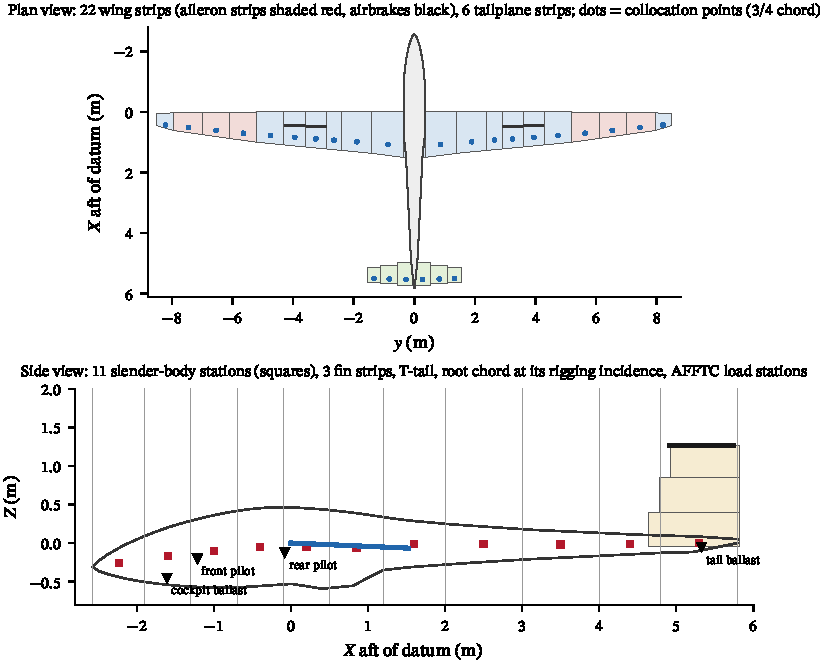
\includegraphics[width=\textwidth]{geometry}
\caption{\vnine{} discretisation drawn from the generator's data. Wing chords, leading-edge line and dihedral come from the
three-view, and are scaled to the type-certificate area of 17.95\,m$^2$ (the drawing integrates to 18.06\,m$^2$). Collocation (3/4-chord)
points carry the lift magnitude; forces act at the 1/4-chord points. Fuselage stations carry slender-body loads. Triangles mark the AFFTC load stations.}
\label{fig:geometry}
\end{figure*}
The planform was digitised from the three-view at 1500\,units/m: 17.0\,m span, straight leading edge, double-tapered trailing edge,
4$^\circ$ dihedral, aileron from 5.20 to 7.95\,m semispan, and an airfoil change from FX\,S\,02-196 at the kink to FX\,60-126 at
the tip (Fig.~\ref{fig:geometry}). The rigging checks of the flight manual~\cite{fmweb} (45, 36 and 13\,mm over 1470, 1000 and 590\,mm gauges)
set the root chord 1.75$^\circ$ above the tailplane, with $+0.31^\circ$ wash-in at the kink, $-0.49^\circ$ washout at the aileron's
outer end and $-0.6^\circ$ extrapolated to the tip. The root chord lies at 2.48$^\circ$ to the body $x$-axis of the JSBSim/FlightGear
frame (2.6$^\circ$ to the horizontal of the three-view), so the tailplane sits at $+0.73^\circ$.
\emph{Ground attitude.} The manufacturer's rigging drawing~\cite{fmweb}, drawn in the levelled attitude, shows the nose- and main-wheel
bottoms level to within 1\,cm over their 2.25\,m spacing. In the body frame this puts the nose-wheel contact 1.9\,cm above the
main-wheel contact; the FlightGear gear and 3-D model have it 7.3\,cm above, which tilts the glider about 1.4$^\circ$ further nose-down
on its wheels. \vnine{} uses the corrected contact (the 3-D model's nose wheel is lowered by the same 5.4\,cm), so it rests at
\NgroundNine$^\circ$ pitch instead of \NgroundFg$^\circ$, with the wing root about 3$^\circ$ instead of 1.7$^\circ$ to the runway.
The independent three-view~\cite{threeview} implies 4.3$^\circ$ and is the outlier. Integrating the
fuselage contours of the side, top and front views with a super-elliptic section factor of 0.82 gives length 8.38\,m,
volume 2.18\,m$^3$, and wetted area 13.5\,m$^2$. The skin-friction build-up uses the manufacturer's 12.33\,m$^2$.
Control travels follow from the rigging data: aileron $+10.8/-26.5^\circ$, elevator $+16.2/-22.6^\circ$, rudder $\pm27.8^\circ$.

\begin{table}[t]
\centering\small
\caption{Mass properties: empty-aircraft inertias and agreement with the 24 AFFTC loadings (each model's own moment arms).}
\label{tab:mass}
\resizebox{\columnwidth}{!}{\Tab{massprops}}
\end{table}

\begin{figure}[t]
\centering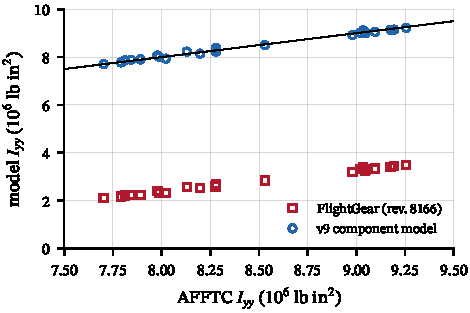
\includegraphics[width=\columnwidth]{inertia}
\caption{Pitch inertia of the 24 AFFTC loadings: model vs.\ measured.}\label{fig:inertia}
\end{figure}
\vnine{} places the occupants and ballast at the AFFTC arms (front seat $-47.91$\,in, rear seat $-3.15$\,in, tail ballast
209.8\,in, cockpit ballast $-63.39$\,in) and uses the measured empty inertias. The test-programme variant carries the
test glider's 851\,lb empty weight. \FG{} keeps Aeromatic estimates that are smaller by factors of 3.1 to 6.5
(Table~\ref{tab:mass}, Fig.~\ref{fig:inertia}). The AFFTC found spin susceptibility to depend on $I_{yy}$ as well as on CG (\ref{eq:inc}--\ref{eq:sus}), so \FG{} starts with a handicap
for the spin map. Together with its weaker roll damping, its small $I_{xx}$ also shortens the roll time constant
fourfold (Table~\ref{tab:modes}).

% =====================================================================================================================
\section{The \vnine{} aerodynamic model}\label{sec:model}
All forces are computed per element in body axes from the local air velocity
\begin{equation}
\mathbf v_i = \mathbf v_\text{air} + \boldsymbol\omega\times(\mathbf r_i-\mathbf r_\text{CG}),
\end{equation}
summed, and referred to the aerodynamic reference point. JSBSim then transfers them to the current CG. Rotation about the CG
therefore enters every strip exactly, which is the essential ingredient for spins and rolls at large rates.

\subsection{Wing: strip theory with an explicit lifting line}
Each of the 22 strips $k$ has a geometric section angle $\alpha_{g,k}$ from the flow at its 3/4-chord point, rotated into the
dihedral plane, plus the local incidence. Induced angles follow from a Weissinger-type influence matrix $\mathsf F$ (trailing
vortex sheets of all strips at the collocation points), with $\Gamma_j=\tfrac12 c_j V_j c_{l,j}$ and
$\alpha_{i,k}=\sum_j F_{kj}\Gamma_j/V_k$. JSBSim's function graph must be acyclic, so the implicit system cannot be iterated.
It is linearised about the section slope $a$ and solved once, offline:
\begin{equation}
\begin{gathered}
\boldsymbol\alpha_i = (\mathsf I + a\,\mathsf F_c)^{-1}\mathsf F_c\,\bigl[c_l(\alpha_g)\,V\bigr]\big/V,\\
\mathsf F_c = \tfrac12\,k_\text{ind}\,\mathsf F\,\mathrm{diag}(c).
\end{gathered}
\label{eq:ll}
\end{equation}
The nonlinear $c_l(\alpha_g)$ inside the bracket keeps the operator consistent at moderate stall, and a fade to zero between
$|\alpha_g|=25^\circ$ and $70^\circ$ removes it in fully separated flow. With $a=6.7$\,rad$^{-1}$ the 22-strip operator gives
$C_{L_\alpha}=5.95$\,rad$^{-1}$ and a Trefftz-plane efficiency $e=1.06$. The value above one is a discretisation artefact,
removed by $k_\text{ind}=1.07$ (converged strip count). Ground effect multiplies $\boldsymbol\alpha_i$ by
$\phi=(16h/b)^2/[1+(16h/b)^2]$~\cite{mccormick}.
The resulting section force is normal and tangential to the local velocity \emph{at the bound vortex} (1/4 chord, Kutta--Joukowski),
whereas the 3/4-chord flow only sets its magnitude. The two differ by $qc/2V$ under a pitch rate (Section~\ref{sec:review}).

\subsection{Sections}
Pre-stall data come from NeuralFoil (``xxlarge'') at the strip Reynolds number, with the profile drag scaled as
$c_d\propto\mathit{Re}^{-0.22}$ for off-design speed. Above $0.8\,c_{l,\max}$ the lift follows a monotone trailing-edge-stall
shape to a peak $k\,c_{l,\max}^\text{NF}$ at $\alpha_\text{peak}$, then drops by $\Delta c_l$ over 5$^\circ$. The lift removed by early
separation reappears as pressure drag. Beyond $\alpha_\text{peak}+b_\text{off}$ the data blend over $d_\text{stall}$ degrees
into a flat plate,
\begin{equation}
\begin{aligned}
c_N&=C_{N,90}\sin(\alpha+k_\delta\delta\cos^2\alpha),\\
x_{cp}&=0.25+(x_{cp,90}-0.25)\,|\alpha|/90^\circ,
\end{aligned}
\end{equation}
with reverse-flow handling up to $\pm180^\circ$ (Fig.~\ref{fig:sections}). The decisive addition for departure behaviour is the
\emph{chordwise} force. Attached flow carries leading-edge suction, $c_A<0$. Once the section has stalled, $c_A$ is blended within
$w_{ca}$ degrees from its value at the lift peak to a small positive value, while $c_N$ is kept:
\begin{equation}
\begin{aligned}
c_A(\alpha) &= (1-s)\,c_A(\alpha_\text{pk}) + s\,\max\bigl(c_A,\;c_{A,\text{sep}}\cos\alpha\bigr),\\
s&=S\bigl((\alpha-\alpha_\text{pk})/w_{ca}\bigr),
\end{aligned}
\end{equation}
where $S$ is a smoothstep. Without this term a stalling wing that drops keeps pulling itself forward and yaws \emph{away}
from the drop; with it, the dropping wing's force tilts aft and yaws it into the spin, as observed.

\begin{figure*}[t]
\centering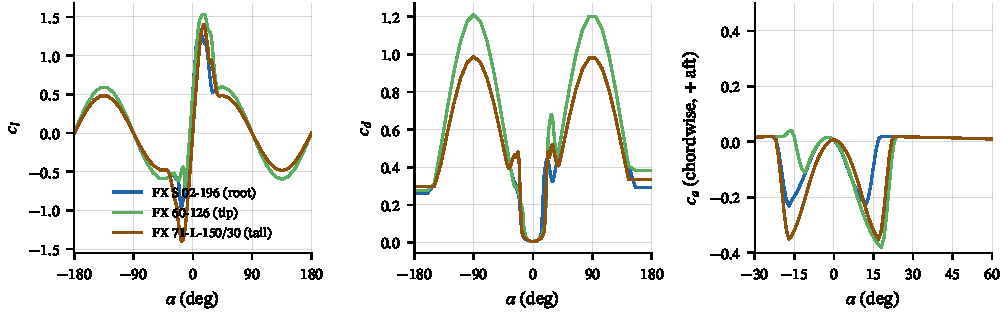
\includegraphics[width=\textwidth]{sections}
\caption{\vnine{} section data (fitted parameters) over $\pm180^\circ$, and the chordwise force $c_A$ with the collapse of leading-edge suction after the stall (right).}
\label{fig:sections}
\end{figure*}

\subsection{Controls and airbrakes}
Ailerons, elevator and rudder are plain flaps evaluated by NeuralFoil on the deflected geometry. Beyond $\pm12^\circ$
NeuralFoil saturates, so the increment curve of the reference deflection is scaled by the increment at $\alpha=0$. A Datcom-type
effectiveness factor (fitted: \NparFlap) accounts for gaps and seals. The stick-centred elevator angle is not documented. A linear
linkage would give the mid-travel value of $-3.2^\circ$. The adopted $-6^\circ$ makes the stick-free, trim-neutral aerotow take-off
(manual: ``trim neutral'', ``take off at about 75\,km/h'') lift off at 81\,km/h with two 80\,kg pilots (Table~\ref{tab:takeoff}). The
airbrakes act as section increments $\Delta c_l,\Delta c_d,\Delta c_m$ over 2.9--4.3\,m semispan, with $\Delta c_d$ calibrated to the
manual's 232\,km/h in a 45$^\circ$ dive (flight path 45$^\circ$ below the horizon) at 600\,kg.

\subsection{Tailplane and fin}
The T-tail sees the wing's downwash from the same trailing-vortex model, tabulated against the tail's height above the
convected wake sheet (inclined at $\alpha-\varepsilon$, $\varepsilon\approx0.28(\alpha+7^\circ)$, $\mathrm d\varepsilon/\mathrm d\alpha=0.28$ at
the tail). It includes a lag $l_t/V$ through $\dot\alpha$, an image-vortex ground-effect factor, and a Silverstein-type Gaussian
wake deficit
\begin{equation}
\begin{aligned}
\frac{\Delta q}{q}&=k_w\,\frac{2.42\sqrt{c_d}}{x/c+0.3}\exp\!\Bigl[-0.69\,\frac{h^2}{c_d\,b_w^2}\Bigr],\\
b_w&=0.68\,c\sqrt{x/c+0.15}.
\end{aligned}
\end{equation}
Tailplane and fin induced angles come from one-mode lifting lines (fin effective aspect ratio 2.35 with the T-tail end plate).
The fin additionally loses dynamic pressure in the separated cross-flow wake of the fuselage at large local sideslip.

\subsection{Fuselage and drag build-up}
Eleven stations carry slender-body loads, Munk's potential term plus Allen--Perkins viscous cross-flow~\cite{allen}. In the
vertical plane a station carries
\begin{equation}
F_z = -k\,\rho\,u\,w\,\Delta S-\tfrac12\rho\,c_{dc}\,A_p\,w\,V_c,\qquad V_c=\sqrt{v^2+w^2},
\end{equation}
and correspondingly $F_y$ with $v$ in the lateral plane; $u,v,w$ are the local velocity components, $\Delta S$ the change of the
equivalent section area across the station and $A_p$ its projected area. The potential term equals $q\,\Delta S\sin2\alpha_t$
resolved into the cross-flow plane. The wing's up- and downwash is added to $w$ ($k=k_2-k_1=0.94$ ahead of the maximum section,
$k\,k_\text{aft}$ behind it). Zero-lift drag is $C_f\,\mathit{FF}\,S_\text{wet}$ for the fuselage
($C_f=0.0026$, $\mathit{FF}=1.09$), a gear drag area of 0.010\,m$^2$, and 0.0017 miscellaneous $C_D$.

\subsection{Implementation and parameter identification}
The generator writes 883 JSBSim functions (768\,kB). The model runs at 51\,$\mu$s per frame, 160 times real time at 120\,Hz, against
4.4\,$\mu$s for \FG. Eighteen factors without a source (Table~\ref{tab:params}) were identified with CMA-ES~\cite{cma}, population 12. The objective sums
(a) spin-map misclassifications, softened by the distance to the AFFTC boundary;
(b) deviations of the developed-spin rate, height loss, pitch attitude and its oscillation, airspeed, bank and load factor from the AFFTC ranges;
(c) recovery turns for six inputs at four loadings;
(d) 1-$g$ stall character at four CGs (elevator limit, $g$-break, bucking, wing drop); and
(e) the manual's stall speeds.
Stage~1 (30 generations, stick-centred elevator at mid travel) was followed by a local stage (12 generations, elevator $-6^\circ$,
spin-rate and height-loss weights tripled). After the corrections of Section~\ref{sec:review} the parameters were re-identified in a
third local stage of 12 generations from the stage-2 result. Of its candidates, the one with the best spin-map agreement
(2 misclassifications, objective 12.59) was taken rather than the one with the lowest objective (12.18, 5 misclassifications). Each objective evaluation flies 100 dynamic test points (about 15\,s on 8 cores).

\begin{table*}[t]
\centering\small
\caption{Identified parameters of \vnine{}: bounds and fitted values.}\label{tab:params}
\Tab{params}
\end{table*}

% =====================================================================================================================
\section{The FlightGear reference model}
\FG{} is a classical build-up about a fixed aerodynamic reference point. $C_L(\alpha)$ is tabulated from $-25^\circ$ to $+25^\circ$ (peak 1.51 at
12$^\circ$) and held constant outside, with a C\,172-derived ground-effect table. $C_D=C_{D0}(\alpha)+0.018\,C_L^2$ plus sideslip, elevator and airbrake terms; damping and
cross derivatives are constants ($C_{m_q}=-13.5$, $C_{m\dot\alpha}=-12$, $C_{l_p}=-0.4$, $C_{n_r}=-0.15$, $C_{l_r}=0.15$,
$C_{n_\beta}=0.15$, $C_{l_\beta}=-0.1$, all per rad on its own reference lengths). Effectiveness tables reduce aileron authority beyond
$\alpha=15^\circ$ and elevator authority beyond $20^\circ$. There is no stall asymmetry, no rate dependence of the stall, and no
$\alpha$ dependence of the rotary derivatives, and the inertias are those of Aeromatic (Table~\ref{tab:mass}).

% =====================================================================================================================
\section{Test method}\label{sec:method}
Both models are run in JSBSim~1.3.2 (Python bindings) at 120\,Hz on the same aircraft root. Only the aerodynamics and
the aircraft file differ; the FCS system file is identical. Loadings are defined by the AFFTC pilot, tail-ballast and
cockpit-ballast masses. \FG{} has no cockpit-ballast station, so its cockpit ballast is added to the front pilot.

\paragraph{Static evaluation.} Static coefficients and trims use the full JSBSim model with frozen integrators. JSBSim derives
$\dot\alpha$ from the instantaneous accelerations, which are non-zero at an unbalanced static point. For coefficient curves and
derivatives, each model's $\dot\alpha$ input is therefore replaced by a free property that is set explicitly.
\paragraph{Pilot models.} Proportional--integral attitude and airspeed loops with rate feedback. Wings are held level with
aileron and the ball centred with rudder unless the test prescribes otherwise.
\paragraph{Stall and spin entries} as flown by the AFFTC:
\emph{WL}, the nose is held 10$^\circ$ high until the stall, then full aft stick and full rudder, aileron neutral;
\emph{WL+A}, the same with full aileron into the spin;
\emph{TH}, the ``thermal entry'': full aileron without rudder near the stall, a 1.5\,s pause, then full rudder and aft stick, aileron neutral.
The AFFTC found the last the most repeatable. Pro-spin controls are held for 40\,s.
\paragraph{Classification.} Spinning means $\alpha>25^\circ$ and $|\dot\psi|>30$\,deg/s. A loading is \emph{incipient} if it
accumulates at least one spinning turn, and \emph{sustained} if it accumulates at least five and is still spinning in the last 8\,s.
Its class is the most spin-prone of its three entries.
\paragraph{Recoveries} start 14\,s after the stall from a WL entry. ``Stopped'' means a rotation rate below 25\,deg/s with
$\alpha<16^\circ$ for 1\,s; turns and height loss are counted from the recovery input.
\paragraph{Other tests.} The 45$^\circ$ airbrake dive is a steady glide along a 45$^\circ$ flight path at 600\,kg. The 1-$g$ stall
speed is the lowest airspeed before the break. The sideslip is compared with a trimmed full-airbrake glide at the same airspeed.
Ground attitude is taken after 10\,s at rest; the parked-in-wind test applies a step wind of 15, 25 or 35\,kt from five directions
for 30\,s. The phugoid is excited by a 1.5\,m/s speed disturbance with the stick fixed, at six speeds from 80 to 140\,km/h.
\paragraph{Small-perturbation modes.} Dimensional body-axis derivatives come from central differences of the model's own
forces about a trimmed 90\,km/h glide, with $\dot\alpha$ as a separate input. The resulting state matrices give phugoid damping
ratios of \NphZFg{} (\FG) and \NphZNine{} (\vnine), against \NphzBFg{} and \NphzBNine{} from the nonlinear simulation at the same speed.

% =====================================================================================================================
\section{Results}
\subsection{Static aerodynamics}
\begin{figure*}[t]
\centering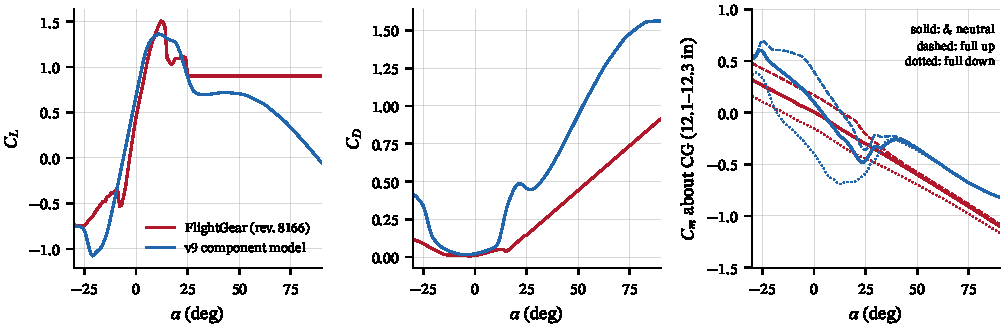
\includegraphics[width=\textwidth]{curves}
\caption{Whole-aircraft static coefficients at 25\,m/s, 2\,$\times$\,80\,kg, $\dot\alpha$ suppressed. \FG{} holds $C_L=0.90$ beyond
25$^\circ$ and has a linear $C_m(\alpha)$ without a stall break; \vnine{} shows the stall break, the post-stall normal force,
and the loss of elevator power beyond $\approx35^\circ$.}
\label{fig:curves}
\end{figure*}
\begin{figure*}[t]
\centering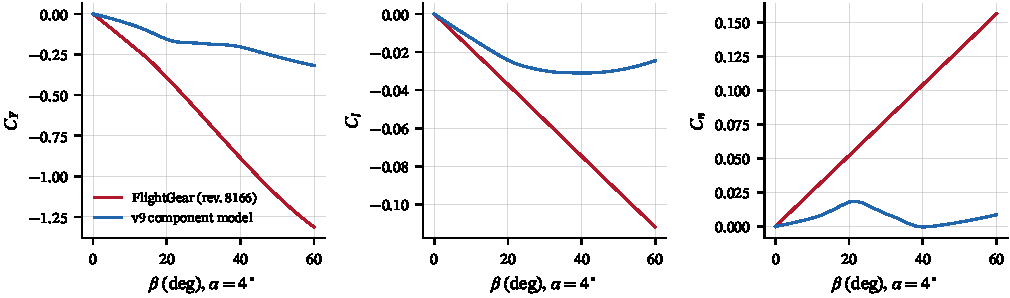
\includegraphics[width=\textwidth]{lateral}
\caption{Lateral--directional static coefficients versus sideslip at $\alpha=4^\circ$. \FG's are linear in $\beta$ to
60$^\circ$. \vnine's yawing moment peaks near 22$^\circ$, where the fin stalls and the fuselage wake starts to blank it,
which is what allows the large full-rudder sideslip of Table~\ref{tab:lateral}.}
\label{fig:lateral}
\end{figure*}
The two models agree on the attached-flow lift slope (\NclaFg{} vs.\ \NclaNine\,rad$^{-1}$ about the respective body axes) but differ
in every respect that matters near and beyond the stall (Figs.~\ref{fig:curves}, \ref{fig:lateral}). \vnine's stall is
gentle ($C_{L,\max}$ \NclmaxNine{} at \NaclmaxNine$^\circ$, falling to \NclThirtyNine{} at 30$^\circ$ before the normal-force regime) and its pitching
moment shows the break that produces the AFFTC's ``very mild $g$-break''. \FG's pitching moment has no stall break.

\subsection{Performance}
\begin{figure*}[t]
\centering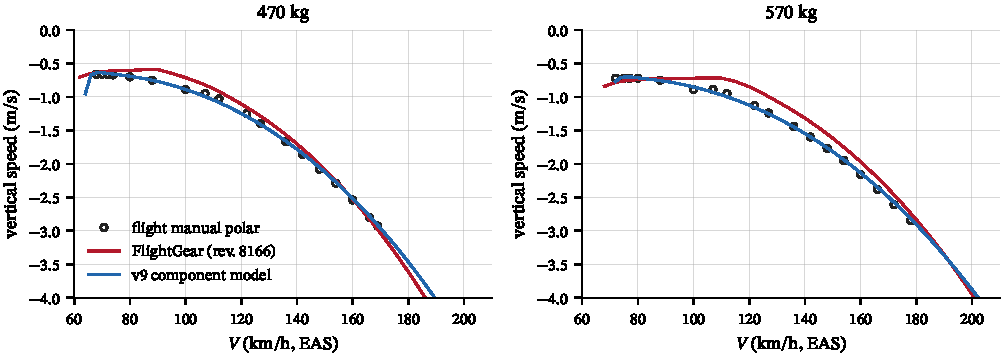
\includegraphics[width=\textwidth]{polar}
\caption{Glide polars against the flight manual (p.~55). Both models are trimmed with the elevator at sea level; the curves are
scaled to the exact manual masses.}
\label{fig:polar}
\end{figure*}
\begin{table}[t]
\centering\small
\caption{Performance against the flight manual. The 45$^\circ$ dive is flown along a 45$^\circ$ flight path at 600\,kg.}\label{tab:perf}
\resizebox{\columnwidth}{!}{\Tab{performance}}
\end{table}
\vnine{} reproduces the manual polar to \NpolRmsNine\,m/s rms at the two masses (Fig.~\ref{fig:polar}, Table~\ref{tab:perf}), with a
best glide of \NldNine{} against 33.5 quoted on the polar and 32.6--33.4 read from its points. \FG{} glides at \NldFg, about 25\,\% better
than the real glider, with its minimum sink at 88--105\,km/h instead of 68--72\,km/h; its induced-drag factor $K=0.018$ corresponds to a span
efficiency of 1.10. The manual's stall speeds of 65 and 74\,km/h come out at \NvsSNine{} and \NvsDNine\,km/h for \vnine{} and
\NvsSFg{} and \NvsDFg\,km/h for \FG. With the airbrakes open the stall speed rises by \NdvsBNine\,km/h in \vnine{} and \NdvsBFg\,km/h in \FG{}
(manual 3\,km/h, AFFTC ``2\,KIAS''). In a 45$^\circ$ dive with the airbrakes open \vnine{} reaches \NdiveNine\,km/h and \FG{} \NdiveFg\,km/h
against the manual's 232\,km/h; for \vnine{} this is a calibration (the airbrake drag increment was set to it), not an independent check.

\subsection{Longitudinal stability and the elevator limit}
\begin{figure}[t]
\centering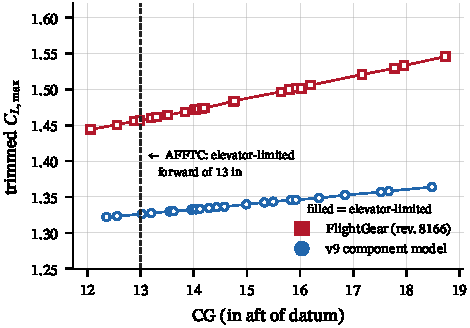
\includegraphics[width=\columnwidth]{clmax}
\caption{Maximum trimmed lift coefficient over the AFFTC loadings.}\label{fig:clmax}
\end{figure}
The stick-fixed neutral point of \vnine{} is at \NnpNine\,in, behind the aft CG limit of 18.46\,in. That of \FG{} is at
\NnpFg\,in (Table~\ref{tab:modes}): \FG{} is statically unstable over the aft 2\,in of the approved CG range, which includes
light solo pilots and 4 of the 24 AFFTC loadings. In \FG{} the lift acts at a fixed reference point and only a constant
$C_{m_\alpha}$ is added, so its neutral point is fixed by construction rather than by the tail.
The AFFTC reports that forward of $\approx13$\,in full aft stick is reached before the stall. Neither model reproduces this
statically (Fig.~\ref{fig:clmax}). In the dynamic 1-$g$ stall at the most forward loading \FG{} does become elevator-limited
(Table~\ref{tab:stall}): it already needs 89\,\% of its up-elevator travel for a static trim at $C_{L,\max}$, and the dynamic entry
uses up the rest. \vnine{} still breaks there, by \NgbreakFwdNine$^\circ$, so its elevator authority at forward CG is too high.

\subsection{Stalls}
\begin{figure*}[t]
\centering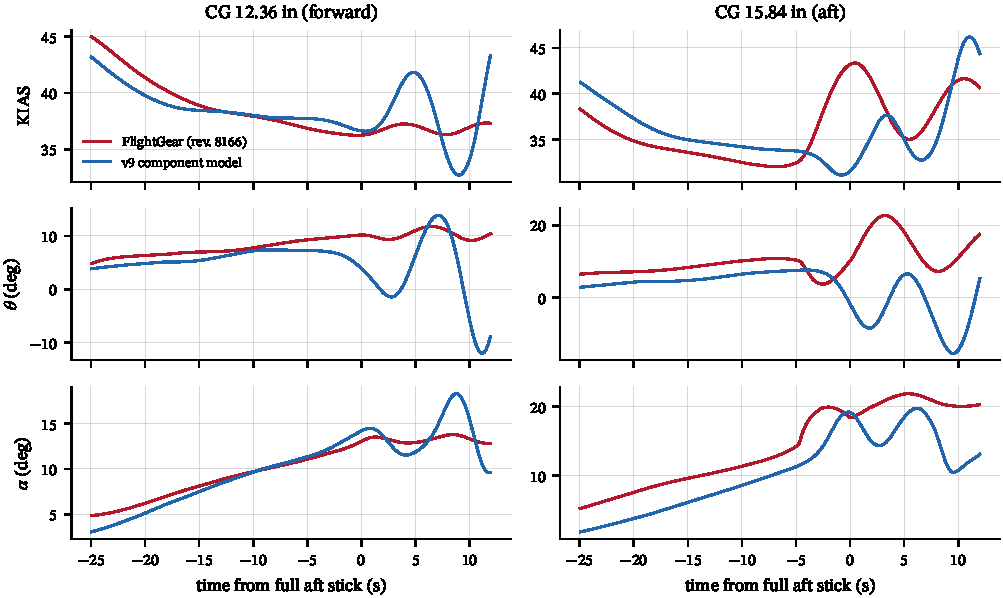
\includegraphics[width=\textwidth]{stall}
\caption{1-$g$ wings-level stalls (deceleration 1\,kt/s, stick then held fully aft for 12\,s) at forward and aft CG.}
\label{fig:stall}
\end{figure*}
\begin{table}[t]
\centering\small
\caption{1-$g$ stalls at four AFFTC loadings. $V_{\min}$ = lowest calibrated airspeed before the break (kt); $g$-break = pitch-attitude drop
within 4\,s after the $\alpha$ peak; bucking = peak-to-peak pitch oscillation with the stick held aft.}
\label{tab:stall}
\resizebox{\columnwidth}{!}{\Tab{stall}}
\end{table}
\begin{table}[t]
\centering\small
\caption{Dynamic (30$^\circ$ nose-high) and inverted stalls; values at the AFFTC loadings 12.36 / 15.83\,in. Height loss with the
scripted recovery (stick released, pull to level flight above 45\,kt).}\label{tab:dynstall}
\resizebox{\columnwidth}{!}{\Tab{dynstall}}
\end{table}
The lowest speeds before the break, \NstallVNine\,kt for \vnine{} and \NstallVFg\,kt for \FG, lie at or slightly below the AFFTC's 33--38\,KIAS
(Fig.~\ref{fig:stall}, Table~\ref{tab:stall}). Aft of 13\,in \vnine{} shows the documented $g$-break followed by pitch bucking, a slow
oscillation as the tail regains power at each nose drop, with no wing drop; its $g$-break of \NgbreakAftNine$^\circ$ is two to three times the
reported 2--3$^\circ$. \FG{} shows no break at its two aft loadings. In the dynamic entry both models reach the reported $\approx20$\,KIAS
(\NpullVNine{} and \NpullVFg\,kt), but \vnine{} drops the nose by \NpullDropNine$^\circ$ against the reported ``up to 40''; height loss
(\NpullHNine\,ft for \vnine, \NpullHFg\,ft for \FG, against $\approx100$\,ft) depends on the scripted recovery. The inverted stall separates
the models clearly: \vnine{} gives \NinvNine\,KIAS (AFFTC 38--40), \FG{} \NinvFg\,KIAS, because its trimmed negative lift peaks at
$C_L$ = \NinvClFg.

\subsection{Spin susceptibility}
\begin{figure*}[t]
\centering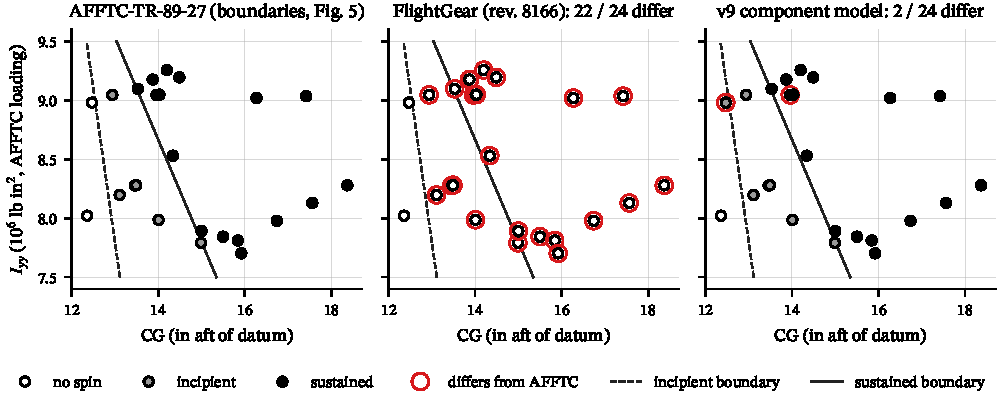
\includegraphics[width=\textwidth]{spinmap}
\caption{Spin susceptibility over the 24 AFFTC loadings, plotted at the AFFTC's CG and $I_{yy}$; boundaries from Eqs.~(\ref{eq:inc})--(\ref{eq:sus}).
Each model loading is classified by its most spin-prone entry (WL, WL+A, TH).}
\label{fig:spinmap}
\end{figure*}
\begin{table}[t]
\centering\small
\caption{\vnine{} loadings classified differently from the AFFTC.}\label{tab:mism}
\Tab{mismatch}
\end{table}
This is the central result (Fig.~\ref{fig:spinmap}). \FG{} does not spin at any of the 24 loadings; it agrees with the AFFTC only at the
\NmatchFg{} loadings forward of the incipient boundary, where no spin is expected. With full pro-spin controls it settles in a spiral dive at
$\alpha$ of 11--20$^\circ$, bank of 50--75$^\circ$, increasing speed and up to 7\,$g$ when aileron is held into the turn (Fig.~\ref{fig:spin}).
The cause is structural: its $C_L$ stays at 0.90 beyond 25$^\circ$ and its roll damping $C_{l_p}=-0.4$ is constant at every $\alpha$, so a
stalled wing never produces the autorotative rolling moment that drives a spin, and its inertias are too small for the inertial pitching
moment that the AFFTC identified as important. \vnine{} classifies \NmatchNine{} of 24 loadings as the AFFTC did. Of the \NmismNine{}
differences (Table~\ref{tab:mism}), \NmismBenign{} are one class too spin-resistant and \NmismProne{} one class too spin-prone; \NmismNear{}
lie within 0.2\,in of a boundary. Of the \NnExpSus{} loadings where the AFFTC obtained sustained spins, \vnine{} sustains a spin with the plain
wings-level entry at \NsusWL, with the thermal entry at \NsusTH{} and with aileron held into the spin at \NsusWLA{} (Appendix~\ref{app:a1}).
The AFFTC found the thermal entry the more successful technique and aileron into the spin to make spins more sustainable.

\subsection{Developed spin}
\begin{figure*}[t]
\centering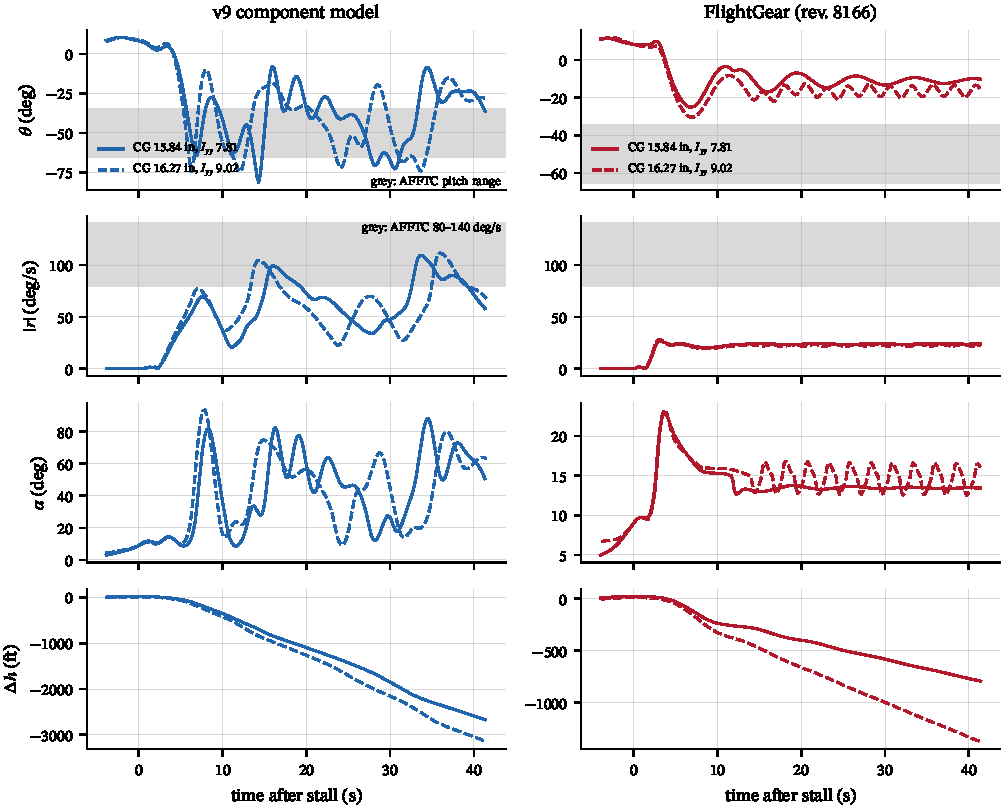
\includegraphics[width=\textwidth]{spin_th}
\caption{Thermal-entry spins at a low-inertia (15.84\,in) and a high-inertia (16.27\,in) loading. Grey bands: AFFTC pitch attitude
(low inertia) and rotation-rate ranges. \FG{} (right) spirals at 20--25\,deg/s with $\alpha$ below 25$^\circ$.}
\label{fig:spin}
\end{figure*}
\begin{table}[t]
\centering\small
\caption{Developed spins: \vnine{} statistics over all sustained spins (from 12\,s after the stall, all entries) against the AFFTC description.}
\label{tab:spinchar}
\resizebox{\columnwidth}{!}{\Tab{spinchar}}
\end{table}
\vnine's developed spin is erect, fast and oscillatory, the AFFTC's modifiers (Fig.~\ref{fig:spin}, Table~\ref{tab:spinchar}). Over its
\NspinN{} sustained spins the mean rate of \NspinRate\,deg/s and \NspinTurn\,s per turn lie inside the reported ranges, and the mean pitch
attitude of \NspinTheta$^\circ$ and mean $\alpha$ of \NspinAlpha$^\circ$ match ``steep''. The oscillation is larger than reported: the pitch
attitude ranges from \NspinThetaMin$^\circ$ to \NspinThetaMax$^\circ$ against $\pm15^\circ$ about $-50^\circ$ (low inertia) or $\pm30^\circ$ about
$-40^\circ$ (high inertia). The mean rate is \NspinRateLo\,deg/s at low and \NspinRateHi\,deg/s at high inertia; the AFFTC found the highest
average rates at forward CG and high inertia. Height loss per turn (\NspinFt\,ft) exceeds the AFFTC's 200\,ft, and the model's mean airspeed
(\NspinKcas\,KCAS) exceeds the indicated 30--40\,KIAS.

\paragraph{How consistent is ``200\,ft per turn''?} With a near-vertical flight path the height loss per turn is
$\Delta h = 2\pi V_z/\Omega$. Equilibrium requires $W=\tfrac12\rho V_z^2 S\,C_v(1+\kappa)$, where
$\kappa=\Omega^2\int c\,y^2\,\mathrm dy/(S V_z^2)$ is the extra dynamic pressure that rotation brings to the outer wing
($\int c\,y^2\,\mathrm dy=327$\,m$^4$). For the AFFTC's nominal values (200\,ft at 105\,deg/s, 8500\,ft altitude, 1150\,lb) these
give $V_z$ = \NparaVz\,m/s TAS (\NparaKt\,kt EAS, consistent with the indicated 30--40\,KIAS), $\kappa$ = \NparaKappa, and a required
vertical-force coefficient $C_v$ = \NparaCv. That is at or above the two-dimensional flat-plate normal force at the spin incidence
($1.98\sin\alpha=1.40$--$1.52$ at 45--50$^\circ$), and above any three-dimensional wing value. \vnine{} develops $C_v$ = \NparaCvNine; its static
resultant coefficient at 45--50$^\circ$ is \NparaCrA. Either the real spin was flatter than its reported attitude, or the altimeter-based
height loss is biased low; a pressure-altimeter lag of a few seconds, for instance, would under-read the height lost over a three-turn spin
by about 150\,ft at a 17\,m/s descent, i.e.\ 50\,ft per turn. The physically plausible value probably lies between 200 and 300\,ft per turn.
Within the present model structure the identification did not find a parameter set that matches the height loss together with the spin map:
it settled on a post-stall normal force of \NparCN{} and a fuselage cross-flow drag coefficient of \NparCdc.

\subsection{Recovery}
\begin{figure*}[t]
\centering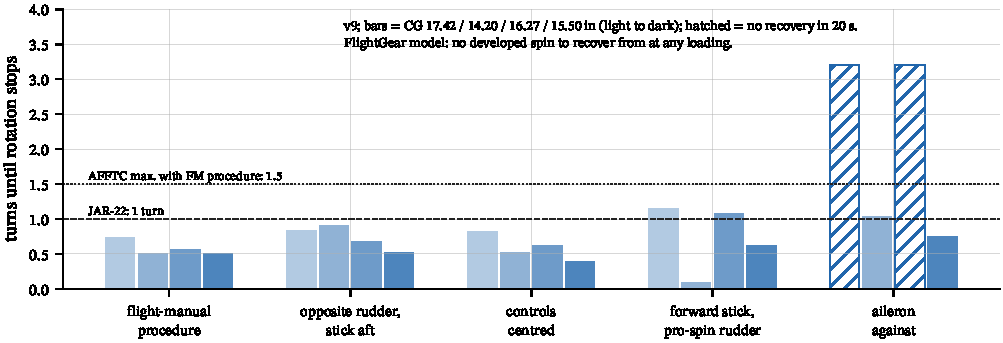
\includegraphics[width=\textwidth]{recovery}
\caption{\vnine{}: turns from the recovery input until the rotation stops.}
\label{fig:recovery}
\end{figure*}
\begin{table*}[t]
\centering\small
\caption{\vnine{} recoveries: turns (height loss) until the rotation stops, at four AFFTC loadings (CG in / $I_{yy}$).
n.s.\ = not spinning at the time of the input; none = no recovery within 20\,s.
\textsuperscript{a}\,The AFFTC released the controls (``hands off''); a free-floating control model would be needed for that test.}
\label{tab:rec}
\Tab{recovery}
\end{table*}
The flight-manual procedure (opposite rudder, a short pause, stick forward) recovers \vnine{} in \NrecFm{} turns, losing \NrecFmFt\,ft until the
rotation stops (AFFTC: 200--300\,ft). Opposite rudder alone, with the stick held aft, recovers in \NrecRud{} turns, against the AFFTC's
$\frac14$--$\frac34$ typical and $1\frac12$ maximum (Fig.~\ref{fig:recovery}, Table~\ref{tab:rec}). Holding the aileron against the spin
fails to recover at \NrecAilNone{} of the \NrecNspin{} loadings, which agrees with ``not a reliable contributor''. Forward stick with
pro-spin rudder recovers \vnine{} after \NrecFwd{} turns; the AFFTC saw up to three additional turns, so \vnine{} is somewhat too benign in
this respect. \FG{} has no spin from which to recover.

\subsection{Lateral--directional handling}
\begin{figure}[t]
\centering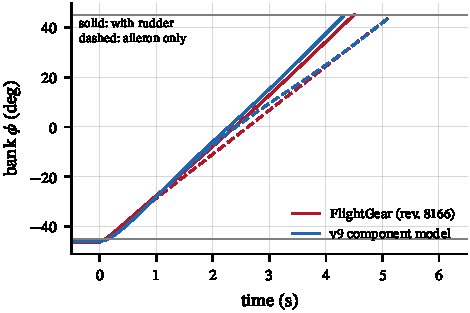
\includegraphics[width=\columnwidth]{roll}
\caption{45$^\circ$--45$^\circ$ roll reversal at 90\,km/h, 2\,$\times$\,80\,kg, full aileron.}\label{fig:roll}
\end{figure}
\begin{figure*}[t]
\centering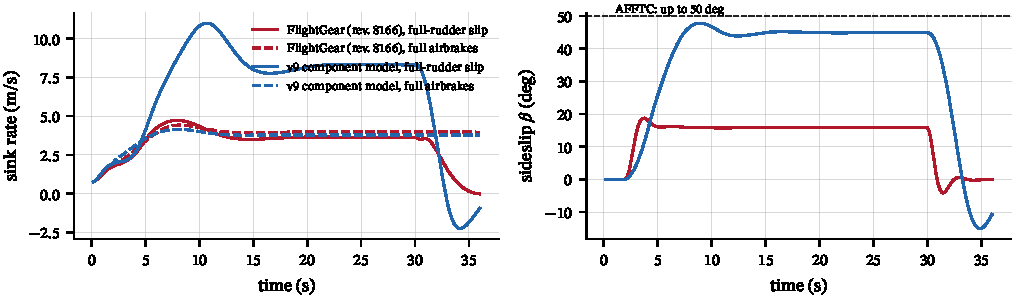
\includegraphics[width=\textwidth]{slip}
\caption{Full-rudder sideslip with the heading held by bank (target 90\,km/h; the slips settle at \NslipVFg{} and \NslipVNine\,km/h CAS), and
a straight glide with full airbrakes.}\label{fig:slip}
\end{figure*}
\begin{table}[t]
\centering\small
\caption{Roll, sideslip and airbrakes. The airbrake sink is taken from a trimmed glide at the airspeed of the slip.
\textsuperscript{b}\,Manual: ``sideslipping is also suitable as an approach control''; the commissioning pilot's experience is that a full slip
is at least as effective as the airbrakes.}
\label{tab:lateral}
\resizebox{\columnwidth}{!}{\Tab{lateral}}
\end{table}
The 45--45$^\circ$ reversal takes \NrollRevNine\,s in \vnine{} and \NrollRevFg\,s in \FG{} with and without rudder (Fig.~\ref{fig:roll});
no measured value is available. A full-aileron roll at the manual's slow-roll entry speeds (165\,km/h dual, 150\,km/h solo) reaches
180$^\circ$ after \NrollHalfNine\,s in \vnine{} and \NrollHalfFg\,s in \FG, against $\approx5$\,s in the flight video. In sideslip
\vnine{} reaches \NslipBetaNine$^\circ$ with full rudder (AFFTC: up to 50$^\circ$) and sinks at \NslipSinkNine\,m/s, \NslipRatioNine{}
times the \NslipBrakeNine\,m/s of a full-airbrake glide at the same airspeed. \FG's linear side-force and yaw derivatives cap the slip at
\NslipBetaFg$^\circ$, where it sinks at \NslipSinkFg\,m/s, less than with airbrakes (\NslipBrakeFg\,m/s). The rudder lock-out reported in
large slips needs a hinge-moment model and is outside both models.

\subsection{Ground attitude and take-off}
\begin{figure*}[t]
\centering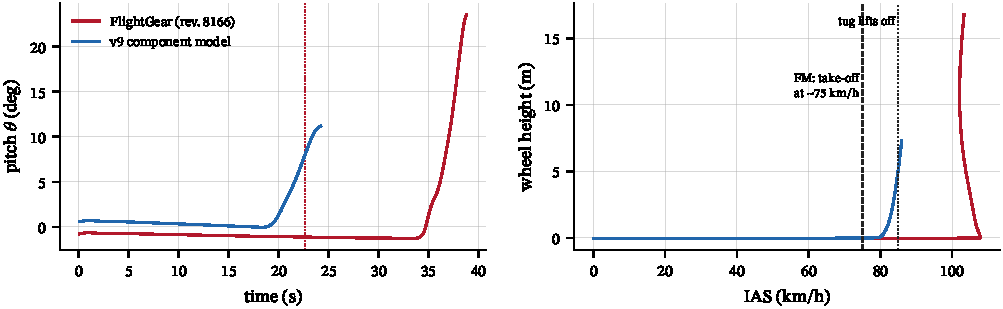
\includegraphics[width=\textwidth]{takeoff}
\caption{Aerotow, 2\,$\times$\,80\,kg, stick centred and trim neutral: 40\,m rope to a tug that accelerates at full power and lifts off at 85\,km/h.}
\label{fig:takeoff}
\end{figure*}
\begin{table}[t]
\centering\small
\caption{Stick-free trim speed (trim neutral) and hands-free aerotow lift-off.
\textsuperscript{c}\,\FG{} has no trim point below the stall with the stick centred at these CGs.}\label{tab:takeoff}
\resizebox{\columnwidth}{!}{\Tab{takeoff}}
\end{table}
On its wheels \vnine{} rests at \NgroundNine$^\circ$ pitch (nose- and main-wheel contacts corrected to the manufacturer's drawing,
Section~\ref{sec:airframe}), \FG{} at \NgroundFg$^\circ$. With the stick centred, a glider lifts off at roughly its stick-free trim speed plus a few km/h
(Fig.~\ref{fig:takeoff}, Table~\ref{tab:takeoff}). \vnine{} lifts off at \NloNine\,km/h for normal loadings, before the tug and close to
the manual's ``about 75\,km/h''; two heavy pilots at the forward limit need a slight pull (\NloHeavyNine\,km/h hands-free). \FG{} lifts off at
\NloFg\,km/h, after the tug, and with the heavy forward loading not at all. The ground-attitude correction alone advances the
hands-free lift-off by only 1--5\,km/h: the nose wheel comes up when the pitching moments balance, which depends on the stick-centred
elevator angle rather than on the wing's angle on the ground. With the mid-travel elevator angle ($-3.2^\circ$) two 80\,kg pilots would lift off
at 88\,km/h, after the tug.

\subsection{Small-perturbation modes}
\begin{figure*}[t]
\centering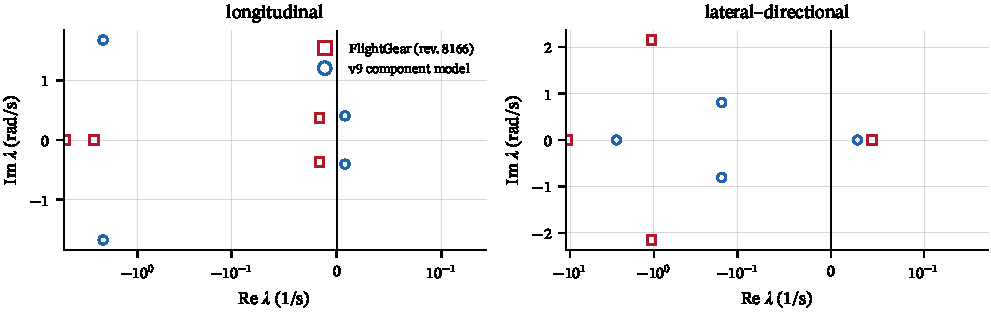
\includegraphics[width=0.85\textwidth]{modes}
\caption{Eigenvalues about a trimmed 90\,km/h glide (2\,$\times$\,80\,kg); symmetric-log real axis.}\label{fig:modes}
\end{figure*}
\begin{table*}[t]
\centering\small
\caption{Non-dimensional derivatives (per rad; $\bar c=1.121$\,m, $b=17$\,m, rates normalised by $\bar c/2V$ and $b/2V$) and modes from the
linearised models. $\tau$ = time constant, $t_2$ = time to double amplitude, $t_{1/2}$ = time to halve it.}
\label{tab:modes}
\Tab{modes}
\end{table*}
\begin{table}[t]
\centering\small
\caption{Phugoid from nonlinear simulation (1.5\,m/s speed disturbance, stick fixed, 2\,$\times$\,80\,kg, CG 12.1--12.3\,in).}
\label{tab:phug}
\resizebox{\columnwidth}{!}{\Tab{phugoid}}
\end{table}
The modes (Fig.~\ref{fig:modes}, Table~\ref{tab:modes}) show the consequences of \FG's mass and damping data. Its roll subsidence
time constant is \NtauRollFg\,s against \NtauRollNine\,s for \vnine{} with the measured $I_{xx}$, and its Dutch roll is a stiff \NdutchFg\,s
oscillation (\vnine: \NdutchNine\,s). \vnine's damping derivatives are close to the classical estimates for this tail volume,
$C_{m_q}\approx-2a_t\eta V_H l_t/\bar c\approx-16$ for the tail alone (\vnine{} \NcmqNine{} in total) and
$C_{m\dot\alpha}\approx C_{m_q}^{\,t}\,\mathrm d\varepsilon/\mathrm d\alpha\approx-4.5$ (\vnine{} \NcmadNine); \FG's \NcmadFg{} is more than twice
that estimate. The phugoid is the one mode where \vnine{} is worse (Table~\ref{tab:phug}). Its damping ratio is negative at low speed,
\NphzANine{} at 80\,km/h (the amplitude doubles within about two cycles) and \NphzBNine{} at 90\,km/h, and turns positive between 100 and
110\,km/h (\NphzDNine{} at 110, \NphzFNine{} at 140\,km/h); \FG's is \NphzBFg{} to \NphzFFg. Both periods exceed Lanchester's
$\pi\sqrt2\,V/g$ (11.3\,s at 90\,km/h) because of the coupling with the pitch damping: without $M_q$ and $M_{\dot\alpha}$ both linear
models return to about 11.5\,s. For a glider of this glide ratio the classical damping is $\zeta\approx1/(\sqrt2\,L/D)\approx0.02$, a small
margin that the derivative sensitivity analysis shows to depend mainly on $M_w$, $M_q$ and $M_{\dot\alpha}$; it gives no single unphysical
cause for the negative value. Measured phugoid damping for the ASK\,21 is not available, but a glider that diverges in pitch within
two oscillations at 80\,km/h would be noticed; this is the most consequential open defect of \vnine{} for normal flying.

\subsection{Robustness}
Both models were parked for 30\,s in 15, 25 and 35\,kt wind from five directions between head- and tailwind, and flown through
60 random upsets ($|\boldsymbol\omega|\le3$\,rad/s, $\alpha$ and attitude anywhere, random controls and wind). All parked runs stayed
finite, with pitch excursions of up to \NwindDthFg$^\circ$ (\FG) and \NwindDthNine$^\circ$ (\vnine) while the glider settled onto a wingtip;
\NfuzzBadFg{} (\FG) and \NfuzzBadNine{} (\vnine) upset runs produced a non-finite state.

% =====================================================================================================================
\section{Summary scorecard}
\begin{table*}[t]
\centering\small
\caption{Behaviour against the sources. \ok\ within the reported range or tolerance; \pok\ qualitatively right, quantitatively off; \nok\ wrong or absent.}
\label{tab:score}
\begin{tabularx}{\textwidth}{@{}Xllrlrl@{}}
\toprule
Criterion & Source & Reference & \multicolumn{2}{c}{FlightGear rev.\ 8166} & \multicolumn{2}{c}{\vnine{}} \\
\midrule
Glide polar, rms sink error & FM p.\,55 & -- & 0.09--0.17\,m/s & \nok & 0.025--0.028\,m/s & \ok \\
Best glide ratio & FM p.\,55 & 33.5 & 42.3--42.5 & \nok & 32.6--32.8 & \ok \\
Stall speed single / dual & FM & 65 / 74\,km/h & 60.3 / 69.3 & \nok & 63.7 / 72.4 & \ok \\
Stall-speed increase, airbrakes & FM, AFFTC & 3\,km/h, 2\,KIAS & 1.0--1.1 & \nok & 2.3--2.6 & \ok \\
Airbrake 45$^\circ$ dive, 600\,kg & FM & 232\,km/h & 194 & \pok & 232 & \ok \\
Neutral point aft of the aft CG limit & -- & $>18.46$\,in & 16.5\,in & \nok & 21.9\,in & \ok \\
1-$g$ stall: forward CG elevator-limited & AFFTC & yes & yes & \ok & no (5.4$^\circ$ break) & \nok \\
1-$g$ stall: aft CG $g$-break + bucking & AFFTC & 2--3$^\circ$, bucking & 0.0--4.0$^\circ$ & \pok & 7.2--7.9$^\circ$ & \pok \\
Dynamic stall: min.\ speed / nose drop & AFFTC & 20\,KIAS / $\le$40$^\circ$ & 21--28 / 0--55$^\circ$ & \pok & 20--25 / 69--76$^\circ$ & \pok \\
Inverted $-1g$ stall & AFFTC & 38--40\,KIAS & 54.4 & \nok & 40.7 & \ok \\
Spin map, 24 loadings & AFFTC Fig.~5 & -- & 2 of 24 & \nok & 22 of 24 & \ok \\
Thermal entry more effective than wings-level & AFFTC & yes & 0 vs 0 & \nok & 11 vs 9 & \ok \\
Spin rate (mean) & AFFTC & 80--140\,deg/s & no spin & \nok & 94 & \ok \\
Spin pitch attitude / oscillation & AFFTC & $-50\pm15^\circ$ (low $I$) & -- & \nok & $-$38, $\sigma$ = 18$^\circ$ & \pok \\
Height loss per turn & AFFTC & 200 (150--250)\,ft & -- & \nok & 313 & \pok \\
Recovery, FM procedure (turns) & FM, AFFTC & $<1$ (max $1\frac12$) & -- & \nok & 0.50--0.73 & \ok \\
Recovery, opposite rudder only (turns) & AFFTC & $\frac14$--$\frac34$ (max $1\frac12$) & -- & \nok & 0.52--0.91 & \ok \\
Forward stick, pro-spin rudder (turns) & AFFTC & up to 3 more turns & -- & \nok & 0.10--1.15 & \pok \\
Full-rudder sideslip & AFFTC & up to 50$^\circ$ & 16$^\circ$ & \nok & 45$^\circ$ & \ok \\
Slip sink vs.\ airbrakes, same speed & FM, pilot & slip $\gtrsim$ brakes & 3.6 vs 4.8\,m/s & \nok & 8.2 vs 5.6\,m/s & \ok \\
Full-aileron roll, first 180$^\circ$ & video & $\approx5$\,s & 6.2--6.6\,s & \pok & 4.4--4.7\,s & \ok \\
Hands-free aerotow lift-off before the tug & FM, pilot & $\approx75$\,km/h & 91--108\,km/h & \nok & 65--79\,km/h & \ok \\
Empty inertias & AFFTC App.~C & 30.2 / 6.7 / 34.3 & 4.6 / 1.4 / 10.9 & \nok & 30.2 / 6.7 / 34.3 & \ok \\
Phugoid damped at 80--140\,km/h & theory & $\zeta\approx0.02$ & min.\ $\zeta$ = 0.06 & \ok & min.\ $\zeta$ = $-$0.06 & \nok \\
\midrule
\multicolumn{7}{p{0.97\textwidth}}{\footnotesize Rules: polar rms $<0.05$\,m/s (\pok\ $<0.10$); best glide 31.5--35 (\pok\ 30--37); stall speeds within 2\,km/h (\pok\ 4); airbrake increment 2--4.5\,km/h; dive within 5\,\% (\pok\ 20\,\%); inverted stall 36--42\,KIAS (\pok\ 32--46); spin map $\ge$20 of 24 (\pok\ $\ge$16); spin rate 80--140; pitch mean $-35$ to $-60^\circ$ with $\sigma\le12^\circ$; height loss 150--250\,ft (\pok\ $\le$350); recoveries $\le1\frac12$ turns; forward stick recovering at all is too benign (\pok); sideslip $\ge35^\circ$ (\pok\ $\ge25^\circ$); roll 4--6\,s (\pok\ 3--7); lift-off below the tug's 85\,km/h with 2\,$\times$\,80\,kg; inertias within 5\,\%; phugoid $\zeta>0$ at all tested speeds. Stall-break rows: \ok\ as described, \pok\ bucking present / break $<3.5^\circ$.} \\
\bottomrule
\end{tabularx}

\end{table*}
Table~\ref{tab:score} condenses the comparison. Of \NscN{} criteria, \FG{} meets \NscOkFg, is qualitatively right in \NscPkFg{} and
fails \NscNoFg; \vnine{} meets \NscOkNine, is qualitatively right but quantitatively off in \NscPkNine{} and fails \NscNoNine.

% =====================================================================================================================
\section{Corrections after the first issue}\label{sec:review}
A first issue of this report contained errors that a line-by-line check against the code and the results files revealed. They are
listed here because three of them changed the model.
\begin{itemize}
\item \textbf{Fuselage potential load.} The slender-body (Munk) term multiplied the \emph{total} dynamic pressure, including the
sideslip component, by $\sin2\alpha$ of the flow in the vertical plane (and vice versa laterally). This inflates the load by $V^2/(u^2+w^2)$:
by up to $\approx20\,\%$ in spins, and without bound in pure cross-flow, where it tipped the parked glider onto its nose in a 15\,kt
crosswind gust. The corrected term is $\rho\,u\,w\,\Delta S$ (Section~\ref{sec:model}).
\item \textbf{Force direction.} Section forces were directed normal to the 3/4-chord flow instead of the 1/4-chord flow (bound vortex),
which produced a spurious $X_q\approx+18$\,lbf\,s/rad.
\item \textbf{Nose-gear contact.} See Section~\ref{sec:airframe}; the gear inherited from the FlightGear model rested the glider $\approx1.4^\circ$ too far nose-down.
\item The 18 parameters were re-identified after these corrections (Section~\ref{sec:model}); all results in this issue are for the corrected model.
\item \textbf{Test definitions.} The 45$^\circ$ airbrake dive had been flown at a 45$^\circ$ pitch attitude (a 40$^\circ$ flight path); the
stall speed had been taken at the $\alpha$ peak, which for \FG{} at aft CG lies after its lift has collapsed and had suggested a stall speed
rising toward aft CG; the slip had been compared with an airbrake glide at a different airspeed; the parked-in-wind test had not been run
for \FG; and the phugoid had been characterised at a single speed.
\item \textbf{Text.} Several statements had not been checked against the final results: the direction of the spin-map misclassifications,
the effect of the entry technique, the ground attitude (stated as 1.8$^\circ$ nose-down), the attribution of informal reports, and the
document titles of two sources.
\end{itemize}

% =====================================================================================================================
\section{Discussion and limitations}
\begin{itemize}
\item \textbf{Why \FG{} cannot spin.} Its $C_L$ table is clamped at 0.90 beyond 25$^\circ$ and its roll and yaw damping are constants,
so no combination of $\alpha$ and rate produces a pro-spin rolling moment. Its inertias are 68--85\,\% too small, so the
inertial pitching moment that holds a real spin at a stalled $\alpha$ is missing. These are structural defects, not tuning errors.
\item \textbf{What is fitted and what is predicted.} The 18 identified factors were fitted to the spin map, the spin characteristics,
the recoveries, four 1-$g$ stalls and the manual's stall speeds. Earlier, two drag factors (profile-drag factor 1.00, miscellaneous
$C_D$ 0.0017) were set from the manual polar and the airbrake drag from the manual's dive speed. The stick-centred elevator angle was
chosen for the hands-free take-off. Not fitted to anything, and therefore predictions, are the roll response, the sideslip
capability and the slip sink rate, the airbrake stall-speed increment, the inverted stall, the static and dynamic stability
derivatives and the phugoid.
\item \textbf{Sensitivity of the boundary.} Near the boundary, outcomes change with the entry details: whether the stall coincides with
peak yaw rate, the elevator gearing, the pause length. The AFFTC observed the same (``spin entry success was sensitive to entry pitch
attitude conditions''). Classifications within $\approx0.2$\,in of a boundary should be read as ties.
\item \textbf{Not modelled.} Free-floating controls and hinge moments (hands-off spin behaviour, rudder lock-out in sideslip,
stick-free stability); pitot--static errors (all model speeds are CAS); unsteady stall hysteresis beyond the downwash lag; wing
flexibility (FlightGear's wing-flex animation reads the model's lift but does not feed back).
\item \textbf{Open quantitative gaps in \vnine.} The divergent phugoid below about 105\,km/h; spin height loss and oscillation amplitude;
an aft-CG $g$-break two to three times the reported value; too large a nose drop in dynamic stalls; and a stall break at forward CG,
where the AFFTC found the elevator running out first.
\item \textbf{Assumed values.} The stick-centred elevator angle ($-6^\circ$), the 85\,km/h tug lift-off speed and the 1\,lb tail-weight bracket
are assumptions; the first is justified only by the manual's take-off statement and the commissioning pilot's experience.
\end{itemize}

% =====================================================================================================================
\section{Conclusions}
A lumped-coefficient model of Aeromatic origin, even one tuned to look right in cruise, cannot reproduce the stall and spin
behaviour of a training sailplane. In the case studied, the FlightGear reference model glides 25\,\% too well, is statically unstable at
aft CG, and turns every spin attempt into a spiral dive. A component build-up from public geometry, airfoil and mass data, closed by a
small number of physically bounded post-stall factors, does markedly better. It matches the manual's polar within the reading accuracy of
the chart and the manual's stall speeds within a few km/h, reproduces \NmatchNine{} of the 24 AFFTC spin classifications including their
dependence on pitch inertia, and reproduces the documented recovery characteristics, the large sideslip capability and the hands-free
take-off. Its remaining errors are quantified: the most consequential for normal flying is a phugoid that diverges at low speed; the
largest against the spin data is the height loss per turn, which sits next to an apparent inconsistency in the reference data itself.

\appendix
\section{Per-loading spin outcomes}\label{app:a1}
\begin{table*}[t]
\centering\small
\caption{All 24 AFFTC loadings: pilot masses (lb), number of tail / cockpit ballast weights, $I_{yy}$ ($10^6$\,lb\,in$^2$), the AFFTC
expectation (Eqs.~\ref{eq:inc}--\ref{eq:sus}) and each model's outcome per entry technique (I = incipient, S = sustained, small
numbers = spinning turns within 40\,s; -- = no spin).}
\label{tab:a1}
\Tab{a1}
\end{table*}
Table~\ref{tab:a1} lists every spin test point.

\section{Reproducibility}
The model generator (\texttt{genxml.py}, \texttt{genjsb.py}, \texttt{airfoils.py}, \texttt{liftingline.py},
\texttt{geometry.py}), the identification (\texttt{objective.py}, \texttt{optimize.py}, \texttt{optimize2.py}) and the test
campaign with its evaluation (\texttt{campaign.py}, \texttt{summarize.py}, \texttt{figures.py}, \texttt{mktables.py},
\texttt{mknumbers.py}, \texttt{paradox.py}) are shipped with the model. \texttt{campaign.py <model>} flies the \NnTests{} test points of
this report; every number in the text and tables is taken from its output by \texttt{mktables.py} and \texttt{mknumbers.py}, except
the reference values and the verdicts of the scorecard. The identified parameter set is \texttt{v9\_params.json}.

\begin{thebibliography}{99}\small
\bibitem{afftc} Air Force Flight Test Center, \emph{Schleicher ASK-21 Glider (TG-9) Stall and Spin Evaluation}, AFFTC-TR-89-27, Edwards AFB, CA, July 1989.
\bibitem{fm04b} Alexander Schleicher GmbH \& Co., \emph{Flight Manual ASK\,21}, US edition incl.\ TN\,4b (2012), with spin-ballast supplement.
\bibitem{fm23} Alexander Schleicher GmbH \& Co., \emph{ASK\,21 Flight Manual}, edition of April 1980 with TN\,23.
\bibitem{mi} Alexander Schleicher GmbH \& Co., \emph{Flughandbuch ASK\,21\,Mi} (flight manual, German), technical data.
\bibitem{fmweb} Alexander Schleicher GmbH \& Co., \emph{Flight Manual ASK\,21}, English edition with pages dated 1983--84 (online copy published by a US soaring club).
\bibitem{threeview} \emph{K21 three view drawing}, vector drawing, 2020, CC\,BY\,4.0.
\bibitem{uiuc} UIUC Applied Aerodynamics Group, \emph{UIUC Airfoil Coordinates Database}, University of Illinois.
\bibitem{neuralfoil} \emph{NeuralFoil: an airfoil aerodynamics analysis tool using physics-informed machine learning}, MIT, 2024 (via AeroSandbox).
\bibitem{jsbsim} JSBSim Development Team, \emph{JSBSim: an open-source flight dynamics model}, version 1.3.2.
\bibitem{aeromatic} Aeromatic, \emph{JSBSim aircraft configuration generator}, version 0.96.
\bibitem{gaeb} Institute of Flight System Dynamics, RWTH Aachen, \emph{Numerical simulation of glider winch launches}, XXX OSTIV Congress, Szeged, 2010.
\bibitem{mccormick} \emph{Aerodynamics, Aeronautics, and Flight Mechanics}, 2nd ed., Wiley, 1995.
\bibitem{allen} NACA, \emph{A study of effects of viscosity on flow over slender inclined bodies of revolution}, NACA Report 1048, 1951.
\bibitem{cma} \emph{The CMA evolution strategy: a tutorial}, arXiv:1604.00772, 2016.
\end{thebibliography}
\end{document}
